% Review-II Presentation -- built on R2_UG_Project_Presentation_Template.tex
% Compile with pdfLaTeX (Overleaf default). Needs ssn-logo.png and figures/
% in the same project. Items in red must be filled in before the review.

\documentclass[aspectratio=169,11pt]{beamer}

% ---------- Theme and colours ----------
\usetheme{Madrid}
\usecolortheme{default}
\definecolor{UniversityBlue}{RGB}{16,62,110}
\definecolor{AccentBlue}{RGB}{30,136,229}
\definecolor{LightBlue}{RGB}{232,242,252}
\definecolor{DarkGray}{RGB}{55,65,81}
\definecolor{DoneGreen}{RGB}{27,122,61}
\definecolor{PlanOrange}{RGB}{194,98,0}

\setbeamercolor{structure}{fg=UniversityBlue}
\setbeamercolor{palette primary}{bg=UniversityBlue,fg=white}
\setbeamercolor{palette secondary}{bg=AccentBlue,fg=white}
\setbeamercolor{frametitle}{bg=UniversityBlue,fg=white}
\setbeamercolor{block title}{bg=UniversityBlue,fg=white}
\setbeamercolor{block body}{bg=LightBlue,fg=black}
\setbeamercolor{alerted text}{fg=AccentBlue}

% ---------- Packages ----------
\usepackage[T1]{fontenc}
\usepackage[utf8]{inputenc}
\usepackage{lmodern}
\usepackage{graphicx}
\usepackage{booktabs}
\usepackage{array}
\usepackage{tabularx}
\usepackage{tikz}
\usetikzlibrary{positioning,arrows.meta}
\usepackage{amsmath}
\usepackage{listings}
\usepackage{xcolor}
\usepackage{colortbl}
\usepackage{hyperref}
\usepackage{pgfgantt}

% ---------- General settings ----------
\setbeamertemplate{navigation symbols}{}
\setbeamertemplate{caption}[numbered]
\setbeamertemplate{itemize item}{\color{AccentBlue}$\blacktriangleright$}
\setbeamertemplate{itemize subitem}{\color{UniversityBlue}$\bullet$}
\setbeamersize{text margin left=0.7cm,text margin right=0.7cm}

% Footer: project title, institution and slide number
\setbeamertemplate{footline}{%
  \leavevmode%
  \hbox{%
    \begin{beamercolorbox}[wd=.42\paperwidth,ht=2.7ex,dp=1.1ex,leftskip=.6em]{author in head/foot}%
      \insertshorttitle
    \end{beamercolorbox}%
    \begin{beamercolorbox}[wd=.46\paperwidth,ht=2.7ex,dp=1.1ex,center]{date in head/foot}%
      Department of Computer Science and Engineering
    \end{beamercolorbox}%
    \begin{beamercolorbox}[wd=.12\paperwidth,ht=2.7ex,dp=1.1ex,center]{page number in head/foot}%
      \insertframenumber/\inserttotalframenumber
    \end{beamercolorbox}%
  }%
  \vskip0pt%
}

% ---------- Code style ----------
\lstset{
  basicstyle=\ttfamily\scriptsize,
  keywordstyle=\color{UniversityBlue}\bfseries,
  commentstyle=\color{gray},
  stringstyle=\color{AccentBlue},
  numbers=left,
  numberstyle=\tiny\color{gray},
  frame=single,
  breaklines=true,
  showstringspaces=false
}

\newcommand{\todo}[1]{\textcolor{red}{[#1]}}
\newcommand{\done}{\textcolor{DoneGreen}{\textbf{Completed}}}
\newcommand{\planned}{\textcolor{PlanOrange}{\textbf{Planned}}}

% ---------- Editable project details ----------
\title[AD Progression Staging from rs-fMRI]{Assessment of Alzheimer's Disease Progression Using a
Comorbidity-Aware Meta-Bayesian Framework with Resting-State fMRI}
\subtitle{Second Review}
\author[Student Team]{%
  Harishkanna R \todo{Register No.}\\
  \todo{Student Name 2 (Register No.)}\\
  \todo{Student Name 3 (Register No.)}
}
\institute[SSN]{%
  Guided by: \todo{Dr. Guide Name, Designation}\\[2mm]
  Department of Computer Science and Engineering\\
  Sri Sivasubramaniya Nadar College of Engineering
}
\date{Academic Year 2026--2027}

\begin{document}

% 1. Title slide
\begin{frame}[plain]
  \titlepage
  \begin{tikzpicture}[remember picture,overlay]
    \node[anchor=south east,xshift=-0.4cm,yshift=0.3cm]
    at (current page.south east){
\includegraphics[width=1.9cm]{ssn-logo.png}};
  \end{tikzpicture}
\end{frame}

% Outline
\begin{frame}{Outline}
  \begin{columns}[T,onlytextwidth]
    \column{0.48\textwidth}
      \begin{enumerate}
        \item First review -- queries and answers
        \item Problem statement and objectives
        \item Dataset
        \item Proposed system architecture
        \item Modules and methodology
      \end{enumerate}
    \column{0.48\textwidth}
      \begin{enumerate}\setcounter{enumi}{5}
        \item Core processing logic
        \item Implementation status
        \item Results and analysis
        \item Plan for the remaining work
        \item References
      \end{enumerate}
  \end{columns}
\end{frame}

% First Review Queries - Answers
\begin{frame}{First Review -- Queries and Answers}
  \small
  \begin{tabularx}{\textwidth}{>{\bfseries}p{4.6cm}X}
    \toprule
    Query & Answer \\
    \midrule
    \todo{Query 1 raised by the panel} & \todo{Answer} \\
    \todo{Query 2 raised by the panel} & \todo{Answer} \\
    \todo{Query 3 raised by the panel} & \todo{Answer} \\
    \bottomrule
  \end{tabularx}
\end{frame}

\begin{frame}{Design Revisions Since Review I}
  \begin{itemize}
    \item \textbf{Feature matrix is $246\times3$, not $246\times4$:}
          FC strength $=$ DC$/245$ exactly ($r=1.0$), so it adds no information.
    \item \textbf{Validation unit is the subject:} 165 scans come from only
          \textbf{127 subjects}; MCI has 32 scans but just 14 subjects.
    \item \textbf{No AD scan is unrecoverable:} the 6 scans once listed as lost
          were found and processed (25/25).
    \item \textbf{Stage order fixed:} CN $\rightarrow$ SMC $\rightarrow$ EMCI
          $\rightarrow$ MCI $\rightarrow$ LMCI $\rightarrow$ AD.
    \item \textbf{Comorbidities named honestly:} ADNI history gives broad
          cardiovascular / endocrine categories, not ``hypertension'' or ``diabetes''.
  \end{itemize}
\end{frame}

% Problem statement
\begin{frame}{Problem Statement}
  \begin{alertblock}{Problem}
    Most rs-fMRI studies only separate \textbf{AD from healthy controls}. Clinicians
    need to know \textbf{where on the six-stage continuum} a person is, with an
    honest \textbf{measure of confidence}.
  \end{alertblock}
  \vspace{0.3cm}
  \begin{columns}[T,onlytextwidth]
    \column{0.5\textwidth}
      \textbf{Task}
      \begin{itemize}
        \item Input: rs-fMRI scan(s) + comorbidity record
        \item Output: ordinal stage $y \in \{$CN, SMC, EMCI, MCI, LMCI, AD$\}$,
              its probability distribution and uncertainty
      \end{itemize}
    \column{0.46\textwidth}
      \textbf{Constraints}
      \begin{itemize}
        \item BOLD only: no T1w image, no slice timing
        \item Mixed TRs (3.0\,s, 2.25\,s, 6.02\,s)
        \item 127 subjects, as few as 14 per class
      \end{itemize}
  \end{columns}
\end{frame}

% Objectives
\begin{frame}{Project Objectives}
  \small
  \renewcommand{\arraystretch}{1.35}
  \begin{tabularx}{\textwidth}{>{\bfseries}p{0.4cm}X>{\centering\arraybackslash}p{2.0cm}}
    \toprule
    \# & \textbf{Objective} & \textbf{Status}\\
    \midrule
    1 & To curate an analysis-ready \textbf{ADNI rs-fMRI cohort} over six stages, documenting every exclusion & \done\\
    2 & To build a reproducible, \textbf{BOLD-only preprocessing pipeline} with per-scan QC & \done\\
    3 & To extract and \textbf{independently verify} ALFF, ReHo, FC and DC on the Brainnetome-246 atlas & \done\\
    4 & To produce a \textbf{leakage-free}, model-ready feature set & \done\\
    5 & To develop a \textbf{comorbidity-aware Meta-Bayesian ordinal model} with uncertainty & \planned\\
    6 & To evaluate it under \textbf{subject-grouped cross-validation} and explain its predictions & \planned\\
    \bottomrule
  \end{tabularx}
\end{frame}

% Dataset
\begin{frame}{Dataset: ADNI Resting-State fMRI}
  \begin{columns}[T,onlytextwidth]
    \column{0.58\textwidth}
      \small
      \begin{tabular}{lrrr}
        \toprule
        \textbf{Group} & \textbf{Eligible} & \textbf{Processed} & \textbf{Subjects}\\
        \midrule
        CN   & 29 & 27 & 26\\
        SMC  & 32 & 31 & 21\\
        EMCI & 30 & 29 & 26\\
        MCI  & 35 & 32 & 14\\
        LMCI & 22 & 21 & 20\\
        AD   & 25 & 25 & 20\\
        \midrule
        \textbf{Total} & \textbf{173} & \textbf{165} & \textbf{127}\\
        \bottomrule
      \end{tabular}
    \column{0.38\textwidth}
      \begin{block}{Accounting}
        \small
        \begin{itemize}
          \item 175 raw scans audited
          \item 29 recovered from raw DICOM
          \item 2 excluded (truncated, duplicate)
          \item 8 rejected: TR $=6.02$\,s breaks the 0.10\,Hz band (Nyquist 0.083\,Hz)
        \end{itemize}
      \end{block}
  \end{columns}
\end{frame}

% Architecture
\begin{frame}{Proposed System Architecture}
  \centering
  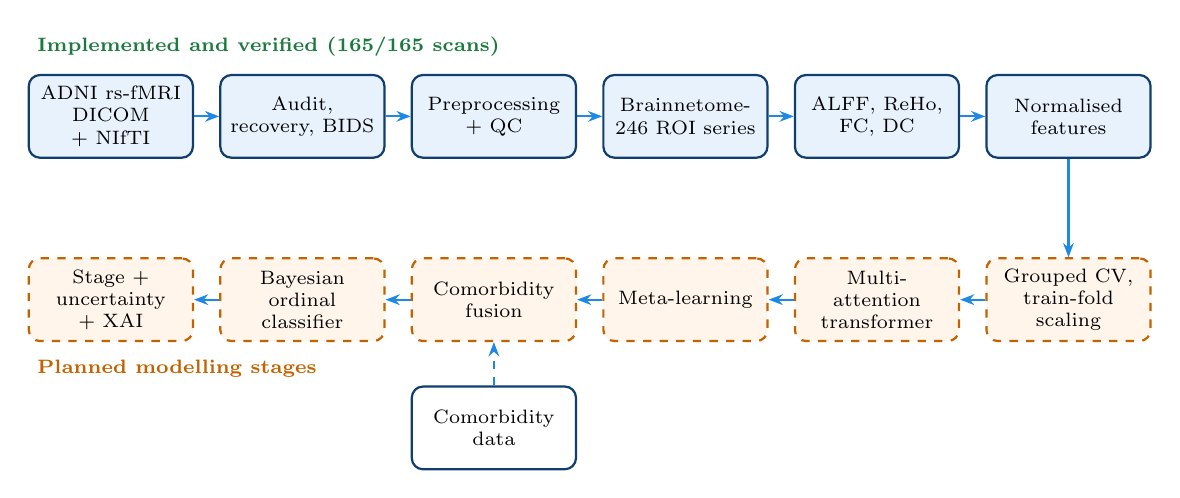
\begin{tikzpicture}[
      >={Stealth[length=1.8mm]},
      box/.style={draw=UniversityBlue,fill=LightBlue,rounded corners,thick,
                  text width=1.85cm,minimum height=1.05cm,align=center,font=\scriptsize},
      plan/.style={box,dashed,draw=PlanOrange,fill=orange!8},
      com/.style={box,fill=white},
      arrow/.style={->,thick,draw=AccentBlue}]
    \node[box] (a1) {ADNI rs-fMRI\\ DICOM + NIfTI};
    \node[box,right=0.32cm of a1] (a2) {Audit, recovery, BIDS};
    \node[box,right=0.32cm of a2] (a3) {Preprocessing + QC};
    \node[box,right=0.32cm of a3] (a4) {Brainnetome-246 ROI series};
    \node[box,right=0.32cm of a4] (a5) {ALFF, ReHo, FC, DC};
    \node[box,right=0.32cm of a5] (a6) {Normalised features};
    \node[plan,below=1.25cm of a6] (b1) {Grouped CV, train-fold scaling};
    \node[plan,left=0.32cm of b1] (b2) {Multi-attention transformer};
    \node[plan,left=0.32cm of b2] (b3) {Meta-learning};
    \node[plan,left=0.32cm of b3] (b4) {Comorbidity fusion};
    \node[plan,left=0.32cm of b4] (b5) {Bayesian ordinal classifier};
    \node[plan,left=0.32cm of b5] (b6) {Stage + uncertainty + XAI};
    \node[com,below=0.55cm of b4] (c) {Comorbidity data};
    \foreach \x/\y in {a1/a2,a2/a3,a3/a4,a4/a5,a5/a6,a6/b1,b1/b2,b2/b3,b3/b4,b4/b5,b5/b6}
      \draw[arrow] (\x) -- (\y);
    \draw[arrow,dashed] (c) -- (b4);
    \node[font=\scriptsize\bfseries,text=DoneGreen,above=0.1cm of a1.north west,anchor=south west]
      {Implemented and verified (165/165 scans)};
    \node[font=\scriptsize\bfseries,text=PlanOrange,below=0.1cm of b6.south west,anchor=north west]
      {Planned modelling stages};
  \end{tikzpicture}
\end{frame}

% Modules
\begin{frame}{System Modules}
  \small
  \begin{enumerate}
    \item \textbf{Module 1 -- Data audit and curation:} inventory, DICOM recovery
          (dcm2niix), duplicate audit, exclusions, slice-timing investigation.
    \item \textbf{Module 2 -- Preprocessing:} motion correction, EPI$\rightarrow$MNI,
          smoothing, nuisance regression, band-pass, QC.
    \item \textbf{Module 3 -- Parcellation and biomarkers:} Brainnetome-246,
          ROI time series, ALFF, ReHo, FC, DC + independent checks.
    \item \textbf{Module 4 -- Normalisation:} within-subject mALFF, mReHo,
          DC$_z$, Fisher-$z$ FC $\rightarrow$ $246\times3$ + $246\times246$.
    \item \textbf{Module 5 -- Staging model (planned):} multi-attention transformer,
          meta-learning, comorbidity fusion, Bayesian ordinal head.
    \item \textbf{Module 6 -- Testing and evaluation:} QC, pilot reproduction gate,
          dataset audits; subject-grouped CV for the model.
  \end{enumerate}
\end{frame}

% Methodology
\begin{frame}{Methodology / Workflow}
  \begin{columns}[T,onlytextwidth]
    \column{0.6\textwidth}
      \small
      \begin{enumerate}
        \item Audit ADNI data, recover missing scans, document exclusions
        \item Preprocess all eligible scans with one frozen pipeline
        \item Align Brainnetome-246; extract ALFF, ReHo, FC, DC
        \item Verify independently; normalise within subject
        \item Build subject-grouped CV folds; scale on training folds only
        \item Train transformer + meta-learning + fusion + ordinal head
        \item Evaluate, calibrate and explain
      \end{enumerate}
    \column{0.36\textwidth}
      \begin{block}{Evaluation Metrics}
        \small
        \begin{itemize}
          \item Balanced accuracy
          \item Mean absolute stage error
          \item Quadratic weighted $\kappa$
          \item Expected calibration error
          \item Ablations (no ordinal / no fusion / no meta-learning)
        \end{itemize}
      \end{block}
  \end{columns}
\end{frame}

% Core logic 1: preprocessing
\begin{frame}{Core Processing Logic: Preprocessing Pipeline}
  \centering
  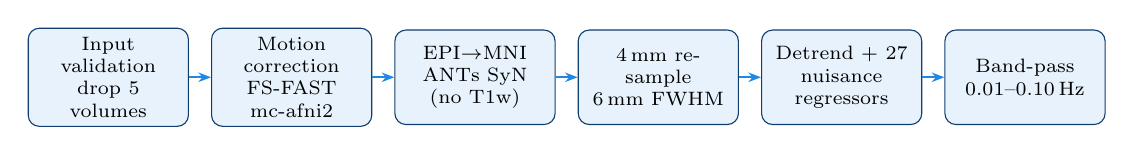
\begin{tikzpicture}[
      >={Stealth[length=1.6mm]},
      st/.style={draw=UniversityBlue,fill=LightBlue,rounded corners,
                 text width=1.8cm,minimum height=1.2cm,align=center,font=\scriptsize},
      arrow/.style={->,thick,draw=AccentBlue}]
    \node[st] (s1) {Input validation\\ drop 5 volumes};
    \node[st,right=0.28cm of s1] (s2) {Motion correction\\ FS-FAST mc-afni2};
    \node[st,right=0.28cm of s2] (s3) {EPI$\rightarrow$MNI\\ ANTs SyN (no T1w)};
    \node[st,right=0.28cm of s3] (s4) {4\,mm resample\\ 6\,mm FWHM};
    \node[st,right=0.28cm of s4] (s5) {Detrend + 27\\ nuisance regressors};
    \node[st,right=0.28cm of s5] (s6) {Band-pass\\ 0.01--0.10\,Hz};
    \foreach \x/\y in {s1/s2,s2/s3,s3/s4,s4/s5,s5/s6} \draw[arrow] (\x) -- (\y);
  \end{tikzpicture}
  \vspace{0.35cm}

  \begin{columns}[T,onlytextwidth]
    \column{0.5\textwidth}
      \begin{block}{Nuisance model (OLS)}
        \small
        Friston-24 motion + WM prior + global signal + intercept.\\
        CSF prior failed the reliability gate in all 165 scans and was dropped,
        not replaced.
      \end{block}
    \column{0.46\textwidth}
      \begin{block}{Never guessed}
        \small
        Slice timing: no metadata $\rightarrow$ not performed.\\
        Nyquist check: $0.10 < 1/(2\,\mathrm{TR})$, else the scan is rejected.
      \end{block}
  \end{columns}
\end{frame}

% Core logic 2: biomarkers
\begin{frame}{Core Processing Logic: Biomarkers and Normalisation}
  \begin{columns}[T,onlytextwidth]
    \column{0.52\textwidth}
      \begin{block}{Biomarkers (per Brainnetome region)}
        \small
        \begin{itemize}
          \item \textbf{ALFF:} mean FFT amplitude in 0.01--0.10\,Hz
          \item \textbf{ReHo:} Kendall's $W$ over a 27-voxel cube
          \item \textbf{FC:} $246\times246$ Pearson, signed, unthresholded
          \item \textbf{DC:} $\mathrm{DC}_i=\sum_{j\ne i}\mathrm{FC}_{ij}$
        \end{itemize}
      \end{block}
    \column{0.44\textwidth}
      \begin{block}{Within-subject normalisation}
        \small
        \begin{itemize}
          \item mALFF $=\mathrm{ALFF}_i/\overline{\mathrm{ALFF}}$
          \item mReHo $=\mathrm{ReHo}_i/\overline{\mathrm{ReHo}}$
          \item DC$_z$: z-score within the scan
          \item FC $\rightarrow \operatorname{artanh}(r)$, diagonal $=0$
        \end{itemize}
      \end{block}
  \end{columns}
  \vspace{0.3cm}
  \begin{alertblock}{Model input per scan}
    \centering $246\times3$ regional matrix (mALFF, mReHo, DC$_z$) $\;+\;$
    $246\times246$ Fisher-$z$ connectivity matrix
  \end{alertblock}
\end{frame}

% Implementation status
\begin{frame}{Implementation Status}
  \small
  \begin{tabularx}{\textwidth}{X>{\centering\arraybackslash}p{2.2cm}X}
    \toprule
    \textbf{Modules} & \textbf{Status} & \textbf{Evidence / Remarks} \\
    \midrule
    M1 Data audit and curation & \done & 175 audited, 29 recovered, 2 excluded \\
    M2 Preprocessing + QC & \done & 165/173 scans; 8 rejected (TR 6.02\,s) \\
    M3 Parcellation + biomarkers & \done & 246/246 ROIs, 165/165 pass checks \\
    M4 Normalisation & \done & 165/165, 0 failures \\
    M5 Staging model & \planned & LMCI comorbidity tables pending \\
    M6 Model evaluation & \planned & Subject-grouped CV protocol fixed \\
    \bottomrule
  \end{tabularx}
  \vspace{0.3cm}

  \footnotesize Stack: Python 3.12, NumPy, SciPy, NiBabel, Nilearn, ANTsPy,
  TemplateFlow, FreeSurfer 7.4.1 (WSL2); single worker with validated
  checkpoint/resume.
\end{frame}

% Screenshots
\begin{frame}{Implementation Output: Per-Scan QC (pilot AD subject)}
  \centering
  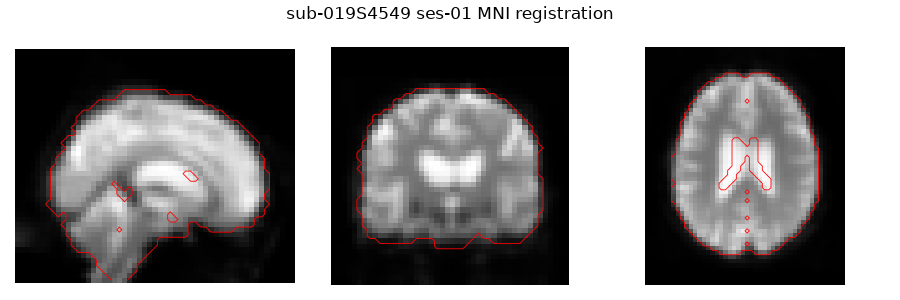
\includegraphics[width=0.66\textwidth]{figures/pilot_registration_qc.png}\\[1mm]
  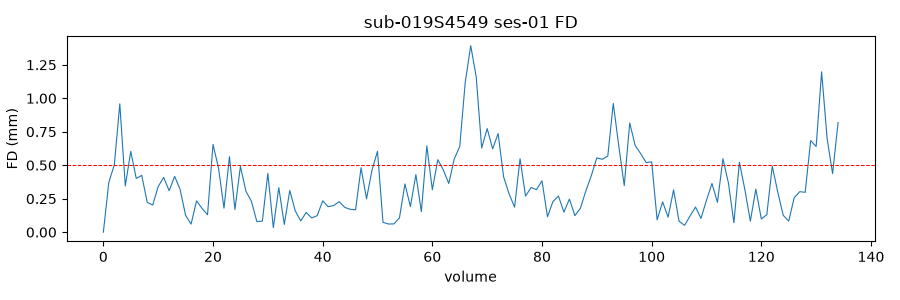
\includegraphics[width=0.66\textwidth]{figures/pilot_fd_plot.png}\\[1mm]
  \footnotesize Top: MNI registration overlay. Bottom: framewise displacement (dashed line 0.5\,mm).
\end{frame}

% Results 1: QC
\begin{frame}{Results: Preprocessing Quality Control}
  \centering
  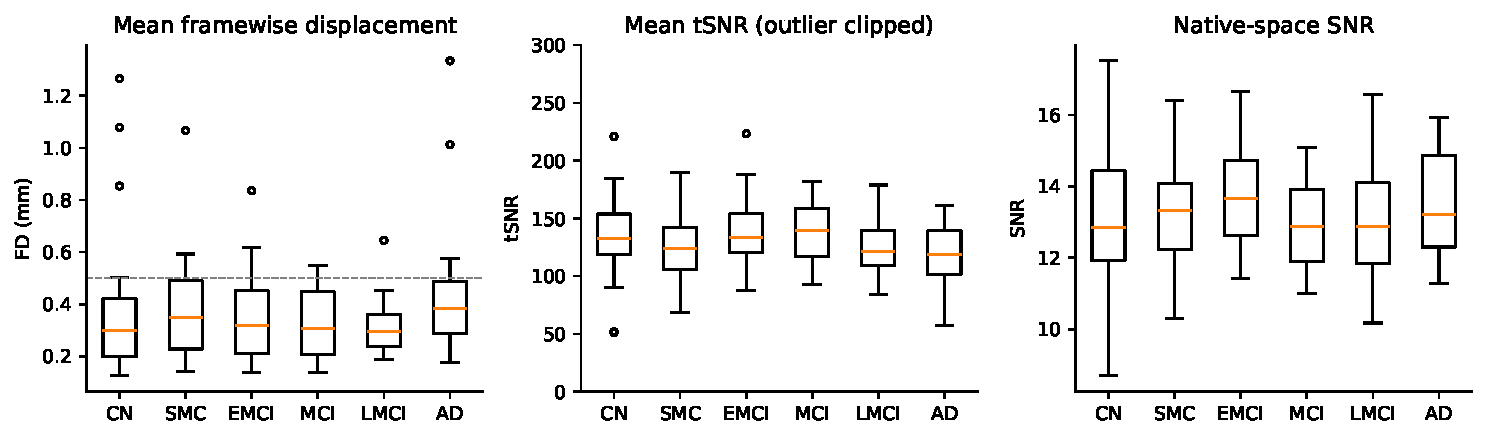
\includegraphics[width=\textwidth]{figures/qc_by_group.pdf}
  \vspace{0.1cm}
  \begin{block}{Key Findings}
    \small
    \begin{itemize}
      \item Median tSNR 119--139 and SNR 12.9--13.8 across groups: no stage-ordered quality bias
      \item AD moves most: mean FD \textbf{0.44\,mm}, 27.7\% of volumes $>0.5$\,mm $\rightarrow$ motion used as a covariate
    \end{itemize}
  \end{block}
\end{frame}

% Results 2: validation
\begin{frame}{Results: Biomarker Verification (all 165 scans)}
  \begin{columns}[T,onlytextwidth]
    \column{0.56\textwidth}
      \small
      \begin{tabular}{lr}
        \toprule
        \textbf{Check} & \textbf{Result}\\
        \midrule
        Scans with 246/246 ROIs & 165/165\\
        ROI series shape $(135,246)$ & 165/165\\
        NaN / Inf / zero-variance & 0 / 0 / 0\\
        ReHo outside $[0,1]$ & 0\\
        FC symmetry error & $2.2\times10^{-16}$\\
        DC recomputed from FC & \textbf{0.000}\\
        Consistent scans & \textbf{165/165}\\
        \bottomrule
      \end{tabular}
    \column{0.40\textwidth}
      \begin{block}{Pilot reproduction gate}
        \small
        Before scale-up, the dataset code had to reproduce the validated pilot:
        ALFF, ReHo, ROI series and atlas labels came back
        \textbf{bit-identical}.\\[1mm]
        Vectorised ReHo: $\sim$68\,s $\rightarrow$ $\sim$3\,s per scan.
      \end{block}
  \end{columns}
\end{frame}

% Results 3: normalisation
\begin{frame}{Results: Why Normalisation and Redundancy Removal}
  \begin{columns}[T,onlytextwidth]
    \column{0.62\textwidth}
      \centering
      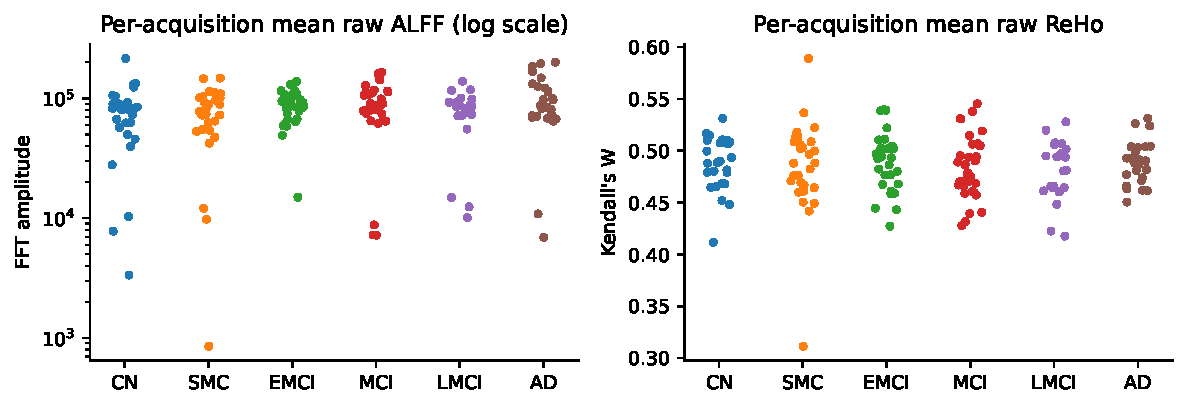
\includegraphics[width=\linewidth]{figures/alff_reho_scaling.pdf}\\
      \footnotesize Raw mean ALFF varies $\sim$250$\times$ between scans
    \column{0.36\textwidth}
      \centering
      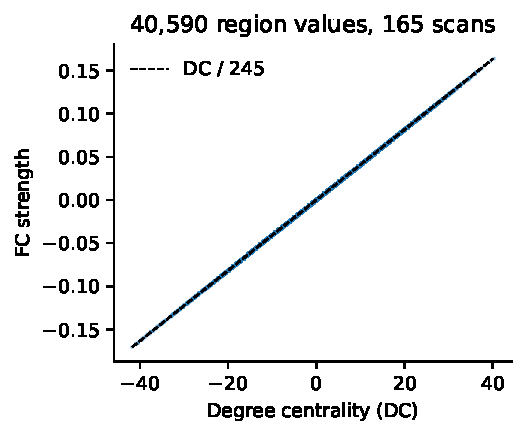
\includegraphics[width=0.92\linewidth]{figures/dc_vs_fcstrength.pdf}\\
      \footnotesize FC strength $=$ DC$/245$ $\Rightarrow$ removed
  \end{columns}
  \vspace{0.2cm}
  \begin{block}{After normalisation}
    \small mean(mALFF) $=$ mean(mReHo) $=$ std(DC$_z$) $=1.000000$ in 165/165;
    Fisher-$z$ diagonal exactly 0; no clipping needed anywhere.
  \end{block}
\end{frame}

% Results 4: group FC
\begin{frame}{Results: Group-Mean Functional Connectivity}
  \begin{columns}[T,onlytextwidth]
    \column{0.64\textwidth}
      \centering
      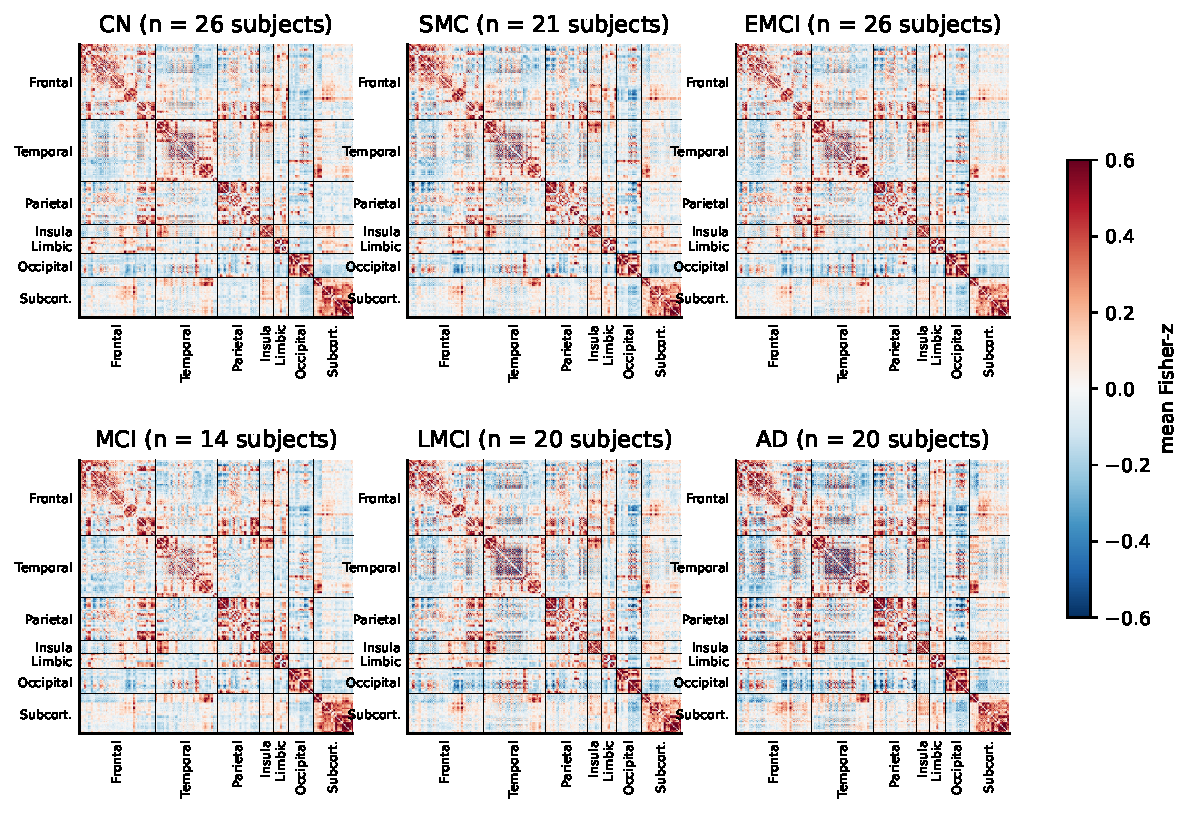
\includegraphics[width=\linewidth]{figures/group_mean_fc.pdf}
    \column{0.33\textwidth}
      \begin{block}{Observation}
        \small
        \begin{itemize}
          \item Same structure in all six groups: strong within-lobe blocks,
                distinct subcortical block
          \item Averaged per subject first (no session inflation)
          \item \textbf{Descriptive only} --- discrimination is the model's job
        \end{itemize}
      \end{block}
  \end{columns}
\end{frame}

% Comparison
\begin{frame}{Comparison with a Conventional Pipeline}
  \small
  \begin{tabularx}{\textwidth}{>{\bfseries}p{3.1cm}XX}
    \toprule
    Aspect & Typical (T1w available) & This project (BOLD-only)\\
    \midrule
    Normalisation & BOLD $\rightarrow$ T1w $\rightarrow$ template & direct EPI $\rightarrow$ MNI (ANTs SyN)\\
    WM/CSF signals & subject tissue segmentation & template priors + reliability gate\\
    Slice timing & corrected from header & not recoverable $\rightarrow$ not performed\\
    Band vs.\ TR & one fixed band & Nyquist checked per scan\\
    Verification & toolbox outputs used directly & exact recomputation, 165/165\\
    Leakage control & whole-dataset scaling common & within-subject; subject-grouped CV\\
    \bottomrule
  \end{tabularx}
\end{frame}

% Plan
\begin{frame}{Plan for the Remaining Work (tentative)}
  \centering
  \begin{ganttchart}[
      hgrid, vgrid,
      x unit=0.36cm, y unit chart=0.42cm,
      title height=1,
      title label font=\scriptsize,
      bar label font=\scriptsize,
      milestone label font=\scriptsize\itshape,
      bar/.append style={fill=AccentBlue!40},
      bar height=0.55,
      milestone/.append style={fill=red!60}]{1}{24}
    \gantttitle{Oct}{4}\gantttitle{Nov}{4}\gantttitle{Dec}{4}
    \gantttitle{Jan}{4}\gantttitle{Feb}{4}\gantttitle{Mar}{4}\\
    \ganttbar{Comorbidity data cleaning}{1}{4}\\
    \ganttbar{Cohort index, grouped CV folds}{3}{5}\\
    \ganttbar{Train-fold scaling, baselines}{5}{8}\\
    \ganttbar{Multi-attention transformer}{7}{12}\\
    \ganttbar{Meta-learning}{11}{15}\\
    \ganttbar{Comorbidity fusion}{13}{16}\\
    \ganttbar{Bayesian ordinal classifier}{15}{18}\\
    \ganttbar{Uncertainty \& explainability}{18}{20}\\
    \ganttbar{Evaluation, ablations, report}{20}{24}\\
    \ganttmilestone{Final review}{24}
  \end{ganttchart}
\end{frame}

% Responsibilities
\begin{frame}{Team Responsibilities}
  \small
  \begin{tabularx}{\textwidth}{>{\bfseries}p{3.3cm}X p{2.3cm}}
    \toprule
    Team Member & Responsibilities & Current Status \\
    \midrule
    Harishkanna R & \todo{Responsibilities} & \todo{Status} \\
    \todo{Student 2} & \todo{Responsibilities} & \todo{Status} \\
    \todo{Student 3} & \todo{Responsibilities} & \todo{Status} \\
    \bottomrule
  \end{tabularx}
\end{frame}

% Conclusion
\begin{frame}{Conclusion}
  \begin{itemize}
    \item The data foundation is \textbf{complete and verified}: 165 scans,
          127 subjects, six stages.
    \item Every BOLD-only limitation is handled by documented exclusion or
          substitution --- \textbf{nothing fabricated}.
    \item Review-I design corrected: \textbf{$246\times3$} features,
          \textbf{subject-level} validation.
    \item Next: comorbidity-aware Meta-Bayesian ordinal model with
          subject-grouped evaluation.
  \end{itemize}
\end{frame}

% References
\begin{frame}[allowframebreaks]{References}
  \footnotesize
  \begin{thebibliography}{9}
    \bibitem{fan2016} L. Fan \emph{et al.}, ``The Human Brainnetome Atlas: A new brain
      atlas based on connectional architecture,'' \emph{Cerebral Cortex},
      vol.~26, no.~8, pp.~3508--3526, 2016.
    \bibitem{zang2007} Y.-F. Zang \emph{et al.}, ``Altered baseline brain activity in
      children with ADHD revealed by resting-state functional MRI,''
      \emph{Brain and Development}, vol.~29, no.~2, pp.~83--91, 2007.
    \bibitem{zang2004} Y. Zang, T. Jiang, Y. Lu, Y. He, and L. Tian, ``Regional
      homogeneity approach to fMRI data analysis,'' \emph{NeuroImage}, vol.~22,
      no.~1, pp.~394--400, 2004.
    \bibitem{zuo2012} X.-N. Zuo \emph{et al.}, ``Network centrality in the human
      functional connectome,'' \emph{Cerebral Cortex}, vol.~22, no.~8,
      pp.~1862--1875, 2012.
    \bibitem{power2012} J. D. Power \emph{et al.}, ``Spurious but systematic
      correlations in functional connectivity MRI networks arise from subject
      motion,'' \emph{NeuroImage}, vol.~59, no.~3, pp.~2142--2154, 2012.
    \bibitem{friston1996} K. J. Friston \emph{et al.}, ``Movement-related effects in
      fMRI time-series,'' \emph{Magnetic Resonance in Medicine}, vol.~35, no.~3,
      pp.~346--355, 1996.
    \bibitem{avants2008} B. B. Avants \emph{et al.}, ``Symmetric diffeomorphic image
      registration with cross-correlation,'' \emph{Medical Image Analysis},
      vol.~12, no.~1, pp.~26--41, 2008.
    \bibitem{vaswani2017} A. Vaswani \emph{et al.}, ``Attention is all you need,''
      in \emph{Advances in Neural Information Processing Systems}, vol.~30, 2017.
    \bibitem{finn2017} C. Finn, P. Abbeel, and S. Levine, ``Model-agnostic
      meta-learning for fast adaptation of deep networks,'' in \emph{Proc. ICML},
      PMLR vol.~70, pp.~1126--1135, 2017.
    \bibitem{mccullagh1980} P. McCullagh, ``Regression models for ordinal data,''
      \emph{J. Royal Statistical Society: Series B}, vol.~42, no.~2,
      pp.~109--142, 1980.
    \bibitem{wen2020} J. Wen \emph{et al.}, ``Convolutional neural networks for
      classification of Alzheimer's disease: Overview and reproducible
      evaluation,'' \emph{Medical Image Analysis}, vol.~63, 101694, 2020.
    \bibitem{adni} Alzheimer's Disease Neuroimaging Initiative (ADNI), 2026.
      [Online]. Available: \url{https://adni.loni.usc.edu}
  \end{thebibliography}
\end{frame}

% Thank you
\begin{frame}[plain]
  \centering
  \vfill
  {\usebeamerfont{title}\color{UniversityBlue}\Huge Thank You}\par
  \vspace{0.5cm}
  {\Large Questions and Discussion}\par
  \vspace{0.8cm}
  \vfill
\end{frame}

\end{document}
